\chapter{Introduction}
\label{introchap}

In the early 1990s it was suggested that linguistics might be the first academic discipline to preside over its own demise. As much as 90\% of the world’s 7,000 languages are predicted to become extinct by the end of the 21st century \citep{krauss_worlds_1992,krauss_keynote--mass_2007,campbell_new_2013}. Therefore, it is critical that languages  be documented and described before they disappear. % without sufficient accessible data.Since the disquieting warning about language endangerment, 
%Linguistic structures and language development cannot be studied without accessible data. 
Linguists have responded by putting greater emphasis on the documentation and description of endangered languages. In the past thirty years, documentary and descriptive fieldwork has achieved impressive results and is steadily broadening our knowledge of the world's language. However, this work 
%including the process of annotating texts and analyzing morphological paradigms, 
is too slow to counteract the crisis of language endangerment. 

If the production of accessible data is to match the pace of language extinction, computational methods must be effectively integrated into the workflow of language documentation and description. Unfortunately, natural language processing (NLP) has not responded as quickly to the language endangerement crisis. Since the 1990s, machine learning systems, capable of learning complex patterns in data, have gained tremendous success in NLP
%Typically, state-of-the-art systems, specifically neural networks, require hundreds of thousands, or even millions, of data instances (words, sounds, sentences, etc.) to achieve state-of-the-art results. Few languages have more than a couple of thousand tokens,
%, let alone much available data, 
but research has been focused on a handful of beyond a handful economically or politically powerful languages such as Chinese, Arabic, English and other European languages. These languages are well documented and described. None 
%demonstrate complicated morphology polysynthetic type, none are under-documented, none 
are endangered.%\mans{The big data requirement is pretty specific to neural models.} 

Fortunately, this is changing. In recent years, NLP research with limited data has burgeoned. This is evidenced, for instance, by the 2015-2019 DARPA-funded LORELEI project, motivated in part by the 2014 Haiti earthquake where disaster aid was hampered by language. Haitian Creole is a language rarely encountered in NLP. When medicine and clean water were available, foreign aid workers struggled to process information that told them where supplies were most urgent. 

Despite this growth, very few NLP systems have been integrated into the process of documenting and describing endangered languages. This may be due to challenges presented by the dynamic, evolving nature of ongoing linguistic analysis and the inconsistencies that arise from manual annotation of data. To overcome these challenges linguists must know how to adjust their methods
%their methods to the specifications of machine learning specifications 
so they can benefit from NLP tools.


\section{Overview of Proposed Research}

\begin{figure}[b]
\centering
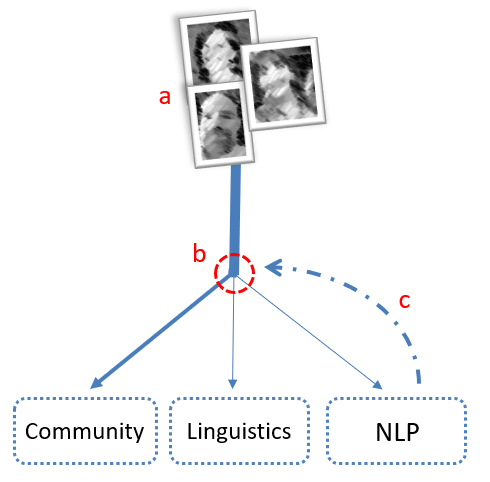
\includegraphics[width=5.75cm]{figs/Flowchart.PNG}
\caption[Language Data Production]{Language Data Production}
\label{fig:flowchart}
\end{figure}

The proposed dissertation research will examine some current language documentation and description methods and investigate how they might be leveraged to more effectively integrate NLP. The general flow of documentary and descriptive work and outcomes is illustrated in Figure \ref{fig:flowchart}. A team of linguists and native speakers (a) collaborate to document and conduct basic linguistic analysis on language data. That data benefits linguistic sciences, NLP development, and the community of speakers. However, because annotating the data is time- and labor-intensive work, a significant portion of that data remains inaccessible (b) to the first two groups, and to a lesser extent, to the community. The proposed dissertation will promote ways to make more data accessible through the integrating NLP systems of machine learning (c). Machine learning can increase %provide automated assistance to document and describe endangered languages with 
speed and accuracy of annotation, but only if linguists know how to make effective use of it. The proposed research 
%will focus on effective integration of machine learning into language documentation and description. It 
will look at ways linguists can adjust their work, specifically as related to interlinearization, so that when machine learning is integrated optimal results are achieved. 
%The proposed research focuses on effective integration for morphological annotation and analysis.

The proposed dissertation is motivated by a “yawning gap” between the amount of documented data deposited in language archives and the portion of the data that is actually usable for research \citep{seifart_language_2018}. This gap is caused by what has been described as an ``annotation bottleneck'', illustrated in Figure \ref{fig:bottleneck}. The bottleneck exists because the accepted annotations methods are tedious, time-consuming, and expensive, performed primarily by hand from start to finish \citep{simons_worlds_2013,holton_developing_2017}.
%The process is labor- and time-intensive. Manual annotation is subject to human error, with many mistakes and inconsistencies due not to the difficulty of the task, but to its repetitive and monotonous nature.
Budget and time constraints often mean that large portions of the data produced by field projects are left unannotated. They remain untapped resources. 
%These resources could inform the development of linguistics science and NLP. They could also build human language technology that would benefit the communities that speak them. 

\begin{figure}[hbt]
    \centering
    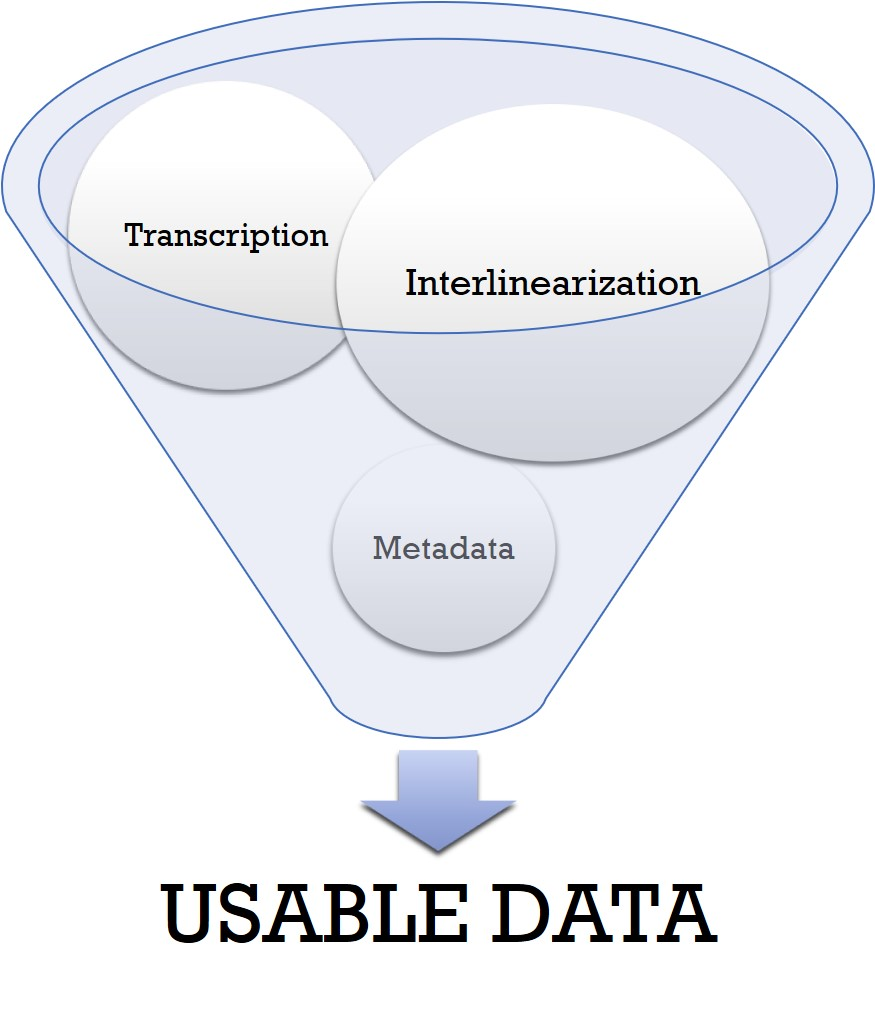
\includegraphics[width=5.5cm]{figs/AnnotationFunnel.jpg}
    \caption[Annotation Bottleneck]{Annotation bottleneck in language documentation and description.}
    \label{fig:bottleneck}
\end{figure}


The proposed dissertation asks: \emph{How would/should the integration of machine learning affect currently accepted workflows of language documentation and description?} It will address the annotation bottleneck by examining how current methods affect machine learning performance and investigating the potential of incorporating machine learning as automated assistance. This will be done with three studies that use NLP machine learning models and documentary and descriptive corpora from seven endangered or under-documented languages.

\begin{enumerate}
\item{} \textbf{Automating Joint Segmentation and Glossing:} How do choices made during interlinearization (i.e. surface versus canonical segmentation, in/consistent manual annotation) affect machine learning results on morpheme segmentation and glossing? How do different machine learning models perform on the data?

%\item{} \textbf{Balance of Interlinearization Tasks:} When faced with limited time, how does integration of machine learning dictate the priorities of completing different interlinear lines? 
%segmentation and glossing over free translation? 
%    \begin{itemize}
%        \item{} What ratio of completed lines achieves optimal machine learning performance on all interlinear lines?
%        \item{} To what extent does completion of other interlinear lines affect the results on any one line? I.e.  Does leveraging glosses improve machine translation? Can information extracted from other lines of interlinear glossed texts improve segmentation and glossing?  
%    \end{itemize}

\item{} \textbf{Morphological Description:} To what extent can manually interlinearized texts be utilized for computational induction of morphological inflection patterns?

\item \textbf{Priority of Part of Speech Tagging:} How should the priorities of part of speech tagging in NLP influence the priorities of documentary and descriptive work?

\end{enumerate}

\section{Expected Results and Implications}

The contribution of the proposed dissertation will be four-fold. 
%study effective integration of computational methods that could open the annotation bottleneck. 
%caused by current time-consuming manual methods to produce morpheme segmentation, glossing, free translation, and first-pass hypotheses of morphological inflectional paradigms. 

First, with successful automated joint segmentation and glossing it will integrate machine learning into the documentary and descriptive pipeline for several typologically different languages. This will demonstrate the potential for producing new annotated data more quickly and accurately than is possible with current methods. While other research has demonstrate this with systems for one or two languages, this research will be conducted on several languages and will show the practicality of automated assistance for morphological annotation regardless of language typology. 

Second, by testing a process to learn inflectional paradigms from field data the proposed dissertation will demonstrate the potential for machine learning to assist linguists in deeper analysis and description. This is a step towards integrating machine learning assistance beyond early documentary stages and using it to build and test holistic hypotheses about a language's structure.

Second, the dissertation will unite the efforts of linguistics and NLP by successfully training machine learning on linguistic field data. A main theme of the proposed research is that machine learning systems can achieve reasonable performance when trained on the often noisy output produced by documentary and descriptive projects. Rather than the curated published data that NLP systems are normally trained on, this research will leverage interlinearized glossed texts from documentary and descriptive field work. Since this research will be performed on ``real live” field data---sometimes the only annotated data available for a language---it may uncover as-yet unforeseen challenges for NLP systems in low-resource settings.
%Specifically, it will use neural networks to learn inflectional patterns in five languages.
%\mans{``neural machine learning'' is perhaps a little too loose: neural networks might be better.}

Third, it will establish not only that new computational methods can be successfully integrated into language documentation and description, but it will show how linguistics field methods may impact NLP systems and test whether certain NLP assumptions about data annotation should impact linguistics field methods. It will do this by studying what happens when NLP priorities are borrowed for documentary and descriptive linguistics, specifically the priority of part of speech (POS) tagging. Additionally, the discussions of other studies will focus on the characteristics and quality of the manually annotated data and how these characteristics affect the machine learning's performance.

Fourth, the proposed research will increase annotated data in five low-resource languages. These languages represent a range of linguistic structures and language families. They are spoken by communities across five continents. Interlinear texts in these languages are currently limited to 5-100K words and the amount of descriptive publications is quite low. Increased annotated data will allow more thorough testing of linguistic theories and computational models.
%, which contribute to our understanding of human language and the performance of machine learning algorithms in low-resource settings. 

\section{Organization of Prospectus}

This Prospectus describes the author's planned dissertation research. Chapter \ref{chap:litreview} reviews issues in previous research that are related to the proposed research. Chapter \ref{chap:datamodels} describes the data and computational models the research will use. Chapter \ref{chap:body} outlines the experiments that will be conducted and presents results from pilot studies. The Prospectus concludes with a timeline (Chapter \ref{chap:timeline}) and a summary and alternative or future work (Chapter \ref{chap:conclusion}).

